%%%%%%%%%%%%%%%%%%%%%%%%%%%%%%%%%%%%%%%%%%%%%%%%%%%%%%%%%%%%%%%%%%%%%%%%%%%%%%%%
\documentclass[paper=a4,fontsize=11pt, hidelinks]{temp} % KOMA-article class
\usepackage[english]{babel}
\usepackage{hyperref} %hyperlinks
\usepackage{fancyhdr}
\usepackage{ifthen} %if then commands
% for header/footer
\pagestyle{fancy}
\renewcommand{\headrulewidth}{0pt} %header separation-line width
\renewcommand{\footrulewidth}{0.4pt} %footer separation-line width
\fancyhead[C]{} %header
\cfoot{ %footer
    In compliance with Italian Legislative Decree n.196 dated 30/06/2003, I hereby authorize to use and process my personal details contained in this document.
    \href{https://igor-lirussi.github.io/Curriculum-Vitae/}{Version updated on \today . \underline{Latest Here}} \\
    \thepage %page number
}

\usepackage{lipsum} %provides filler text

%%%%%%%%%%%%%%%%%%%%%%%%%%%%%%%%%%%%%%%%%%%%%%%%%%%%%%%%%%%%%%%%%%%%%%%%%%%%%%
\begin{document}

% Upload a your photo and rename it to "photo.png" or "photo.jpg"
\begin{minipage}{.2\linewidth}
   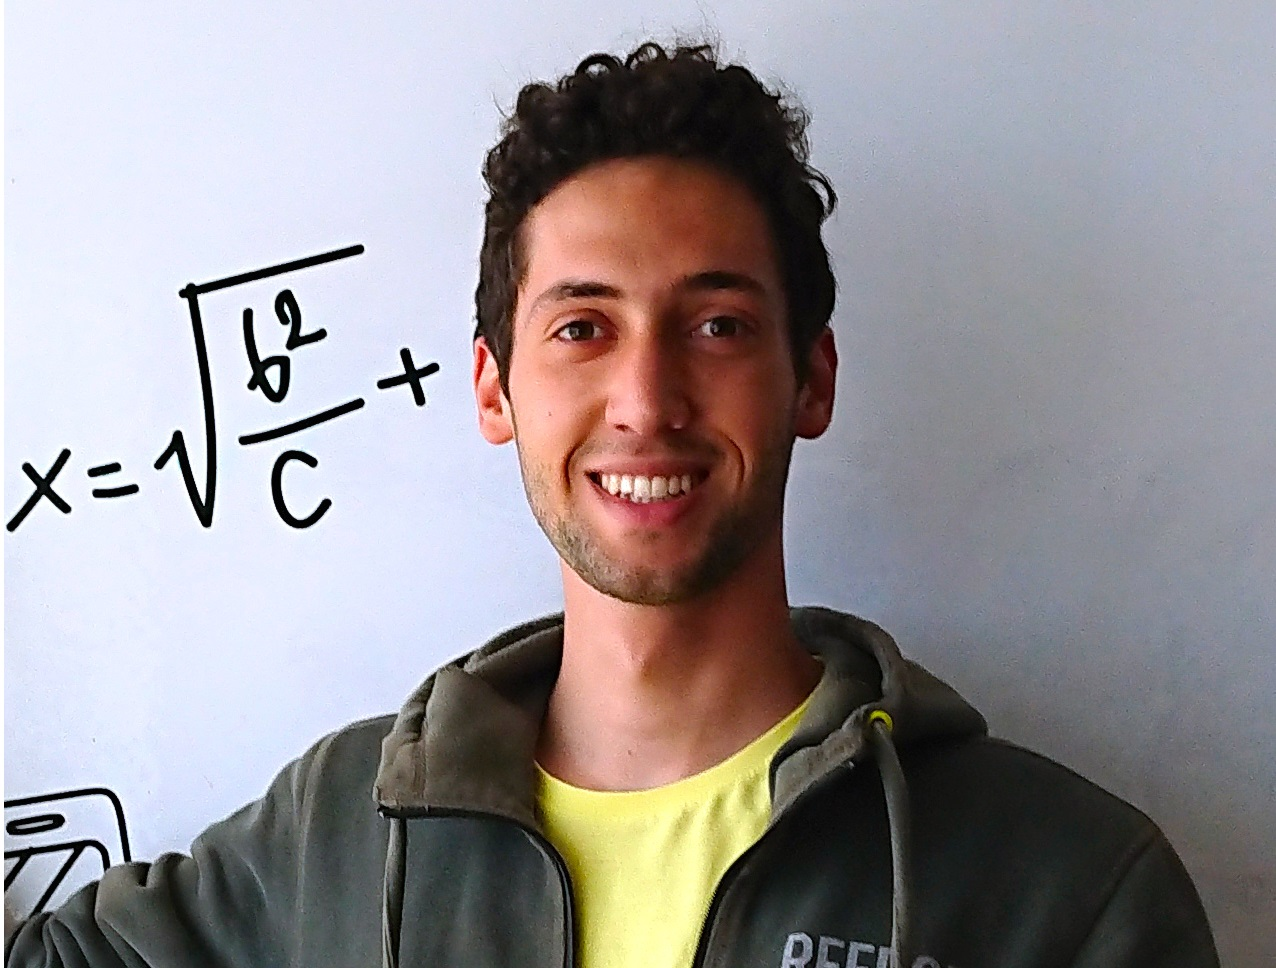
\includegraphics[width=1\textwidth]{photo} %photo
\end{minipage}      
\begin{minipage}{0.7\linewidth}
    \MyName{Igor Lirussi}
    \sepspace
    \noindent
    % info 
    \hfill Gender: M | Nationality: Italian | Marital Status: Single | Birth: 25/12/1995
    
    \hfill \href{mailto:igor.lirussi@studio.unibo.it}{igor.lirussi@studio.unibo.it } | +39 3317055048 
    
    \hfill GitHub/LinkedIn: igor-lirussi | Skype: igor.lirussi
    
    \hfill via VI Maggio, 24, 33030, Forgaria nel Friuli (UD), Italy
 
\end{minipage}


%%%%%%%%%%%%%%%%%%%%%%%%%%%%%%%%%%%%%%%%%%%%%%%%%%%%%%%%%%%%%%%%%%%%%%%%%%%%%%%%
\NewPart{Work Experience}{}
\noindent

\href{https://colors.cmpe.boun.edu.tr}{
\shortEntry{RESEARCH ASSISTANT - COGNITIVE ROBOTICS}
{Oct 2021 - Sep 2022}
{Istanbul (TR) Boğaziçi University: Cognitive Learning and Robotics Laboratory}
{
    \ifthenelse{\isShort=0} {%long version
     \begin{itemize}
        \item Cognitive Robotics
        \item Virtual Reality
     \end{itemize}
    }{%short version
     Cognitive Robotics and Virtual Reality
    } 
} {IMG/bogazici}
}
\sepspace

\href{https://www.kth.se/is/rpl}{
\shortEntry{RESEARCH ASSISTANT - INTERACTION ROBOTICS}
{Apr 2020 - Sep 2020}
{Stockholm (SE) KTH Royal Institute of Technology: Robotic Perception and Learning Department}
{
    \ifthenelse{\isShort=0} {%long version
     \begin{itemize}
        \item Human Robot Interaction
        \item Dialog Engines
     \end{itemize}
    }{%short version
     Human Robot Interaction and Dialog Engines
    } 
} {IMG/kth}
}
\sepspace

\href{https://welcome.isr.tecnico.ulisboa.pt/}{
\shortEntry{RESEARCH SCHOLAR - COMPUTER VISION}
{Sep 2018 - Sep 2019}
{Lisbon (PT) IST Instituto Superior Técnico: I.S.R. Institute for Systems and Robotics - VisLab}
{
    \ifthenelse{\isShort=0} {%long version
     \begin{itemize}
        \item Object recognition and Dialog Processing for Human-Robot Interaction
        \item SLAM and Visual Navigation Systems
     \end{itemize}
    }{%short version
     Object Recognition, NLP for Human-Robot Interaction, SLAM and Visual Navigation Systems
    } 
} {IMG/ist}
}

%%%%%%%%%%%%%%%%%%%%%%%%%%%%%%%%%%%%%%%%%%%%%%%%%%%%%%%%%%%%%%%%%%%%%%%%%%%%%%%%
\NewPart{Education}{}
\noindent

\href{https://corsi.unibo.it/2cycle/ComputerScienceEngineering}{
\longEntry{MSc. COMPUTER SCIENCE AND ENGINEERING}
{Sep 2019 - Today}
{University of Bologna}
{
    \ifthenelse{\isShort=0} {%long version
    Distributed Systems, Machine Learning, Languages, Compilers and Computational Models, Information Systems, Concurrent and Distributed Programming, Programming and Development Paradigms, Web Services and Applications, Smart City and Mobile Technologies, Agile, Continuous Integration and Delivery. 
    }{%short version
    LM-32 - 2nd level-cycle degree in Computer Engineering
    } 
} 
{IMG/unibo}
}
\sepspace

\href{https://dsv.su.se/en/}{
\longEntry{ERASMUS MSc.}
{Jan 2020 - Jul 2020}
{Stockholm University}
{Decision Making and Business Intelligence, Network Security, Cyber Forensics}
{IMG/stockholmuni}
}
\sepspace

\href{https://ciencias.ulisboa.pt/en}{
\longEntry{ERASMUS BSc.}
{Sep 2018 - Sep 2019}
{Lisbon University}
{Artificial Intelligence, Operational Research} 
{IMG/ulisboa}
}
\sepspace

\href{https://corsi.unibo.it/1cycle/ComputerScienceEngineering}{
\longEntry{BSc. COMPUTER SCIENCE AND ENGINEERING}
{Sep 2014 - Sep 2019}
{University of Bologna}
{
    \ifthenelse{\isShort=0} {%long version
    Software Engineering, Embedded Systems and IoT, Automatic Controls, Mobile Application Programming, Operating Systems, Object-Oriented Programming, Network Programming, Telecommunications Networks, Law for Information Technology, Fundamentals of Image Processing, Databases, Algorithms and Data Structures, Computer Architecture, C Programming
    }{%short version
    L-8 - 1st level-cycle degree in Information Technology
    } 
} 
{IMG/unibo}
}

%%%%%%%%%%%%%%%%%%%%%%%%%%%%%%%%%%%%%%%%%%%%%%%%%%%%%%%%%%%%%%%%%%%%%%%%%%%%%%%%
\NewPart{Skills \& Interests}{}
\hspace{3mm}
\begin{minipage}[t]{0.32\textwidth} 
%Languages (ISO 639-1)
\begin{tabular}[t]{ l c l }
\flag{IMG/flag/it}  & IT & Native Speaker \\
\flag{IMG/flag/gb}  & EN & \href{https://github.com/igor-lirussi/Curriculum-Vitae/raw/main/Certificates/IELTS_LIRUSSI.pdf}{Full Proficiency }\\
\flag{IMG/flag/pt}  & PT & \href{https://github.com/igor-lirussi/Curriculum-Vitae/raw/main/Certificates/cert_PT_LIRUSSI.pdf}{Conversational level }\\
\flag{IMG/flag/sv}  & SV & \href{https://github.com/igor-lirussi/Curriculum-Vitae/raw/main/Certificates/cert_SE_LIRUSSI.pdf}{Basic level}\\
%\flag{IMG/flag/de}  & DE & \href{https://github.com/igor-lirussi/Curriculum-Vitae/raw/main/Certificates/cert_DE_LIRUSSI.pdf}{Basic level}\\
\end{tabular}
\end{minipage}
%
\begin{minipage}[t]{0.65\textwidth} 
\begin{tabular}[t]{ l l }
\href{https://site.unibo.it/startupdayunibo/en/programme/the-30-new-emerging-ideas-of-2021}{Winner "The 30 new emerging ideas of 2021" - StartUp Day Unibo}\\
Theoretical and Practical course of First Aid for companies\\
Great Cook and Sport Enthusiast\\
Food Aid Program Volunteer - Blood Donor\\


%\software{IMG/soft/writeL}  	 & Latex Writing\\
%\software{IMG/soft/office} 		 & This software experience. fillertext fillertext fillertex\\
%\software{IMG/soft/Matlab}  	 & This software experience. fillertext fillertext fillertex\\
%\software{IMG/soft/office} 		 & This software experience. fillertext fillertext fillertex\\
%\software{IMG/soft/Matlab}  	 & This software experience. fillertext fillertext fillertex\\
\end{tabular}
\end{minipage}


%%% References

\end{document}
